\documentclass[mathserif]{beamer}
\usepackage{amsmath}
\usepackage{color}
\usepackage{amsfonts}
\usepackage{xcolor,graphicx}
\usepackage{geometry}
\usepackage{hyperref}
\usepackage{mathrsfs}
\usepackage{multimedia}

\title[Primordial Black Holes]{The Effects of a Primordial Black Hole on the Surface of a Neutron Star}
\author{Brady Metherall}
\date{April 13, 2017}

\usetheme[hideothersubsections]{Berkeley}
\usecolortheme{whale}
\definecolor{mycolour}{RGB}{150, 150, 255}
\setbeamercolor{block body}{bg=mycolour,fg=black}

\DeclareMathOperator{\sgn}{sgn}
\DeclareMathOperator{\Heavi}{H}

\DeclareMathOperator{\Hsign}{\mathscr{H}}
\newcommand\Hank[2][]{{\left( \Hsign_{#1} #2 \right) }}

\begin{document}
\frame{\titlepage}
\setlength\parindent{0pt}

\section{Introduction}

\frame{
\frametitle{Black Holes}
\begin{itemize}
\item A black hole is a region of space where enough mass is concentrated such that nothing,
including light, can escape its gravitational pull.
\item Typical black holes form from the collapse of a massive star, and have a minimum mass on the order of a few solar masses.
\item In the early universe while it was very hot and dense, small perturbations could be enough to create small black holes called primordial black holes.
\item The mass of a primordial black hole is probably much less than one solar mass ($10^{-18} - 10^{-6} M_{\odot}$), and microscopic in size.
\end{itemize}
}

\frame{
\frametitle{Primordial Black Holes as Dark Matter}
Dark matter is matter that does not emit/absorb light, and is chargeless. Dark matter accounts for about a quarter of the energy in the universe, but we don't know what it is. \\
\vspace*{\baselineskip}
Primordial black holes may be a good candidate for dark matter since: they are chargeless, do not emit light, have a very small radius, and are non-relativistic. Also, most other proposed explanations of dark matter involve creating a new particle not part of the Standard Model.
}

\section{Model}

\frame{
\frametitle{Flat Star Model}
Investigate the collision of a primordial black hole with a neutron star with the following assumptions:
\begin{itemize}
\item Neutron stars are flat and infinite
\item Primordial black holes are point masses
\item Neutron stars are incompressible fluids
\item Gravitational interactions are Newtonian
\item Primordial black hole has a constant velocity
\end{itemize}
}

\section{Analytic Solution}

\subsection{Velocity Potential}

\frame{
\frametitle{Eigenfunctions of Laplacian}
To find the velocity potential we need the eigenfunctions of the Laplacian. First, assume a product solution and solve the Laplacian.
\begin{align*}
\varphi &= R(r) Z(z) \Theta(\theta) T(t) \\
\nabla^2 \varphi &= 0 \\
\implies \varphi &\propto \left\{ \begin{matrix}J_\mu(kr) \\ Y_\mu(kr) \end{matrix} \right\}  \left\{ \begin{matrix}e^{-kz} \\ e^{kz} \end{matrix} \right\} \left\{ \begin{matrix}\sin(\mu \theta) \\ \cos(\mu \theta) \end{matrix} \right\} T(t) \\
\implies \varphi &\propto J_0(kr) e^{kz} T(t)
\end{align*}
$T(t)$ comes from boundary conditions.
}

\frame{
\frametitle{Hankel Transform}
The Hankel transform is needed to solve the time component of the velocity potential, and the calculation of the energy.
\begin{definition}
\label{def:hanktrans}
The Hankel transform of a function $f(s)$ is given by
\begin{align*}
\Hank[\nu]{f}(\sigma) = \int_0^\infty f(s) J_\nu(s \sigma) s \, ds,
\end{align*}
where $J_\nu$ is the Bessel function of the first kind, of order $\nu \geq -\frac{1}{2}$, and $\sigma$ is a non-negative real variable.
\end{definition}
\begin{corollary}
\label{def:invhanktrans}
The Hankel transform is self-reciprocal, that is, it is its own inverse.
\end{corollary}
}

\frame{
\frametitle{Solving for $\varphi$}
From the pressure condition
\begin{align*}
\left( \frac{\partial^2 \varphi}{\partial t^2} + g \frac{\partial \varphi}{\partial z} + \frac{\partial \Phi}{\partial t} \right) \bigg|_{z=0} = 0.
\end{align*}
We can write the potential as a Hankel transform
\begin{align*}
\frac{\partial \Phi}{\partial t}\bigg|_{z=0} =  \int_0^\infty \Hank{\frac{\partial \Phi}{\partial t}\bigg|_{z=0}}(k) J_0(kr) k \, dk.
\end{align*}
Then,
\begin{align*}
\varphi = \frac{Gmv}{g} \int_0^\infty \frac{J_0(kr)e^{kz}}{1+kv^2/g} \left(-\sgn(t)e^{-kv|t|} + 2 \Heavi(t)\cos(\omega_k t) \right)dk,
\end{align*}
with $\omega_k^2=gk$
}

\subsection{Deformation of Surface}

\frame{
\frametitle{Deformation of Surface}
We can easily solve for the shape of the surface now that we have the velocity potential, using
\begin{gather*}
\frac{\partial \varphi}{\partial z} \bigg|_{z=0} = \frac{\partial \eta}{\partial t}. \\
\eta = \frac{Gm}{g} \int_0^\infty \frac{J_0(kr)}{1+kv^2/g} \left(e^{-kv|t|} + 2\Heavi(t)v \sqrt{\frac{k}{g}} \sin(\omega_k t) \right)dk
\end{gather*}
}

\frame{
\frametitle{Analytic Surface Waves}
\begin{figure}
\centering
\movie[width=8cm, height=6cm,poster, loop, autostart]{}{../Videos/SurfaceWaves.mp4}
\caption{Waves!}
\end{figure}
}

\subsection{Energy}

\frame{
\frametitle{Energy Transferred}
We can calculate the energy by taking the sum of the kinetic, and potential energies,
\begin{align*}
E(t) &= \frac{1}{2}\rho \int_{-\infty}^0 \int_0^\infty |\nabla \varphi |^2 \, r dr dz \int_0^{2\pi} d\theta \\
& \qquad + \rho g \int_0^\infty \int_0^\eta z dz \, rdr \int_0^{2\pi} d\theta \\
\lim_{t \rightarrow \infty} E(t) &= 4 \pi \rho \frac{G^2 m^2}{g}.
\end{align*}
We take the limit as $t$ approaches infinity, because we are interested in the total energy transferred.
}

\frame{
\frametitle{Analytic Energy}
\begin{figure}
% GNUPLOT: LaTeX picture with Postscript
\begingroup
  \makeatletter
  \providecommand\color[2][]{%
    \GenericError{(gnuplot) \space\space\space\@spaces}{%
      Package color not loaded in conjunction with
      terminal option `colourtext'%
    }{See the gnuplot documentation for explanation.%
    }{Either use 'blacktext' in gnuplot or load the package
      color.sty in LaTeX.}%
    \renewcommand\color[2][]{}%
  }%
  \providecommand\includegraphics[2][]{%
    \GenericError{(gnuplot) \space\space\space\@spaces}{%
      Package graphicx or graphics not loaded%
    }{See the gnuplot documentation for explanation.%
    }{The gnuplot epslatex terminal needs graphicx.sty or graphics.sty.}%
    \renewcommand\includegraphics[2][]{}%
  }%
  \providecommand\rotatebox[2]{#2}%
  \@ifundefined{ifGPcolor}{%
    \newif\ifGPcolor
    \GPcolortrue
  }{}%
  \@ifundefined{ifGPblacktext}{%
    \newif\ifGPblacktext
    \GPblacktexttrue
  }{}%
  % define a \g@addto@macro without @ in the name:
  \let\gplgaddtomacro\g@addto@macro
  % define empty templates for all commands taking text:
  \gdef\gplbacktext{}%
  \gdef\gplfronttext{}%
  \makeatother
  \ifGPblacktext
    % no textcolor at all
    \def\colorrgb#1{}%
    \def\colorgray#1{}%
  \else
    % gray or color?
    \ifGPcolor
      \def\colorrgb#1{\color[rgb]{#1}}%
      \def\colorgray#1{\color[gray]{#1}}%
      \expandafter\def\csname LTw\endcsname{\color{white}}%
      \expandafter\def\csname LTb\endcsname{\color{black}}%
      \expandafter\def\csname LTa\endcsname{\color{black}}%
      \expandafter\def\csname LT0\endcsname{\color[rgb]{1,0,0}}%
      \expandafter\def\csname LT1\endcsname{\color[rgb]{0,1,0}}%
      \expandafter\def\csname LT2\endcsname{\color[rgb]{0,0,1}}%
      \expandafter\def\csname LT3\endcsname{\color[rgb]{1,0,1}}%
      \expandafter\def\csname LT4\endcsname{\color[rgb]{0,1,1}}%
      \expandafter\def\csname LT5\endcsname{\color[rgb]{1,1,0}}%
      \expandafter\def\csname LT6\endcsname{\color[rgb]{0,0,0}}%
      \expandafter\def\csname LT7\endcsname{\color[rgb]{1,0.3,0}}%
      \expandafter\def\csname LT8\endcsname{\color[rgb]{0.5,0.5,0.5}}%
    \else
      % gray
      \def\colorrgb#1{\color{black}}%
      \def\colorgray#1{\color[gray]{#1}}%
      \expandafter\def\csname LTw\endcsname{\color{white}}%
      \expandafter\def\csname LTb\endcsname{\color{black}}%
      \expandafter\def\csname LTa\endcsname{\color{black}}%
      \expandafter\def\csname LT0\endcsname{\color{black}}%
      \expandafter\def\csname LT1\endcsname{\color{black}}%
      \expandafter\def\csname LT2\endcsname{\color{black}}%
      \expandafter\def\csname LT3\endcsname{\color{black}}%
      \expandafter\def\csname LT4\endcsname{\color{black}}%
      \expandafter\def\csname LT5\endcsname{\color{black}}%
      \expandafter\def\csname LT6\endcsname{\color{black}}%
      \expandafter\def\csname LT7\endcsname{\color{black}}%
      \expandafter\def\csname LT8\endcsname{\color{black}}%
    \fi
  \fi
    \setlength{\unitlength}{0.0500bp}%
    \ifx\gptboxheight\undefined%
      \newlength{\gptboxheight}%
      \newlength{\gptboxwidth}%
      \newsavebox{\gptboxtext}%
    \fi%
    \setlength{\fboxrule}{0.5pt}%
    \setlength{\fboxsep}{1pt}%
\begin{picture}(5760.00,3844.00)%
    \gplgaddtomacro\gplbacktext{%
    }%
    \gplgaddtomacro\gplfronttext{%
      \csname LTb\endcsname%
      \put(176,2141){\makebox(0,0){\strut{}$E$}}%
      \put(3088,154){\makebox(0,0){\strut{}$\tau$}}%
      \csname LTb\endcsname%
      \put(682,858){\makebox(0,0)[r]{\strut{}$30$}}%
      \csname LTb\endcsname%
      \put(682,2032){\makebox(0,0)[r]{\strut{}$40$}}%
      \csname LTb\endcsname%
      \put(682,3205){\makebox(0,0)[r]{\strut{}$50$}}%
      \csname LTb\endcsname%
      \put(814,484){\makebox(0,0){\strut{}$-30$}}%
      \csname LTb\endcsname%
      \put(1572,484){\makebox(0,0){\strut{}$-20$}}%
      \csname LTb\endcsname%
      \put(2330,484){\makebox(0,0){\strut{}$-10$}}%
      \csname LTb\endcsname%
      \put(3089,484){\makebox(0,0){\strut{}$0$}}%
      \csname LTb\endcsname%
      \put(3847,484){\makebox(0,0){\strut{}$10$}}%
      \csname LTb\endcsname%
      \put(4605,484){\makebox(0,0){\strut{}$20$}}%
      \csname LTb\endcsname%
      \put(5363,484){\makebox(0,0){\strut{}$30$}}%
    }%
    \gplbacktext
    \put(0,0){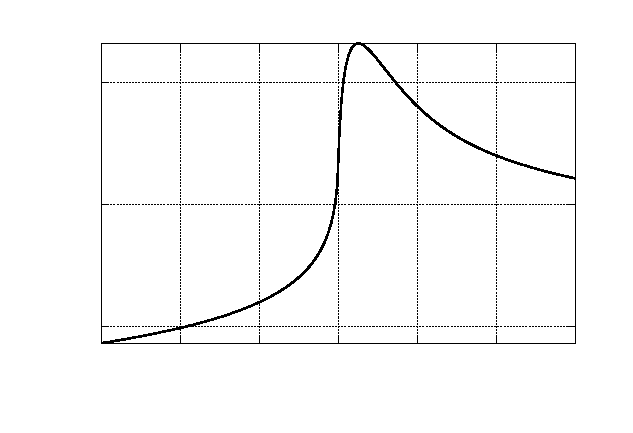
\includegraphics{./AnalyticEnergy}}%
    \gplfronttext
  \end{picture}%
\endgroup

\end{figure}
}

\section{Simulation Solution}

\subsection{Smooth Particle Hydrodynamics}

\frame{
\frametitle{Analytic Surface Waves}
\begin{figure}
\centering
\movie[width=6cm, height=6cm,poster, loop, autostart]{}{../Videos/SimulationWaves.mp4}
\caption{Waves!}
\end{figure}
}

\frame{
\begin{figure}
% GNUPLOT: LaTeX picture with Postscript
\begingroup
  \makeatletter
  \providecommand\color[2][]{%
    \GenericError{(gnuplot) \space\space\space\@spaces}{%
      Package color not loaded in conjunction with
      terminal option `colourtext'%
    }{See the gnuplot documentation for explanation.%
    }{Either use 'blacktext' in gnuplot or load the package
      color.sty in LaTeX.}%
    \renewcommand\color[2][]{}%
  }%
  \providecommand\includegraphics[2][]{%
    \GenericError{(gnuplot) \space\space\space\@spaces}{%
      Package graphicx or graphics not loaded%
    }{See the gnuplot documentation for explanation.%
    }{The gnuplot epslatex terminal needs graphicx.sty or graphics.sty.}%
    \renewcommand\includegraphics[2][]{}%
  }%
  \providecommand\rotatebox[2]{#2}%
  \@ifundefined{ifGPcolor}{%
    \newif\ifGPcolor
    \GPcolortrue
  }{}%
  \@ifundefined{ifGPblacktext}{%
    \newif\ifGPblacktext
    \GPblacktexttrue
  }{}%
  % define a \g@addto@macro without @ in the name:
  \let\gplgaddtomacro\g@addto@macro
  % define empty templates for all commands taking text:
  \gdef\gplbacktext{}%
  \gdef\gplfronttext{}%
  \makeatother
  \ifGPblacktext
    % no textcolor at all
    \def\colorrgb#1{}%
    \def\colorgray#1{}%
  \else
    % gray or color?
    \ifGPcolor
      \def\colorrgb#1{\color[rgb]{#1}}%
      \def\colorgray#1{\color[gray]{#1}}%
      \expandafter\def\csname LTw\endcsname{\color{white}}%
      \expandafter\def\csname LTb\endcsname{\color{black}}%
      \expandafter\def\csname LTa\endcsname{\color{black}}%
      \expandafter\def\csname LT0\endcsname{\color[rgb]{1,0,0}}%
      \expandafter\def\csname LT1\endcsname{\color[rgb]{0,1,0}}%
      \expandafter\def\csname LT2\endcsname{\color[rgb]{0,0,1}}%
      \expandafter\def\csname LT3\endcsname{\color[rgb]{1,0,1}}%
      \expandafter\def\csname LT4\endcsname{\color[rgb]{0,1,1}}%
      \expandafter\def\csname LT5\endcsname{\color[rgb]{1,1,0}}%
      \expandafter\def\csname LT6\endcsname{\color[rgb]{0,0,0}}%
      \expandafter\def\csname LT7\endcsname{\color[rgb]{1,0.3,0}}%
      \expandafter\def\csname LT8\endcsname{\color[rgb]{0.5,0.5,0.5}}%
    \else
      % gray
      \def\colorrgb#1{\color{black}}%
      \def\colorgray#1{\color[gray]{#1}}%
      \expandafter\def\csname LTw\endcsname{\color{white}}%
      \expandafter\def\csname LTb\endcsname{\color{black}}%
      \expandafter\def\csname LTa\endcsname{\color{black}}%
      \expandafter\def\csname LT0\endcsname{\color{black}}%
      \expandafter\def\csname LT1\endcsname{\color{black}}%
      \expandafter\def\csname LT2\endcsname{\color{black}}%
      \expandafter\def\csname LT3\endcsname{\color{black}}%
      \expandafter\def\csname LT4\endcsname{\color{black}}%
      \expandafter\def\csname LT5\endcsname{\color{black}}%
      \expandafter\def\csname LT6\endcsname{\color{black}}%
      \expandafter\def\csname LT7\endcsname{\color{black}}%
      \expandafter\def\csname LT8\endcsname{\color{black}}%
    \fi
  \fi
    \setlength{\unitlength}{0.0500bp}%
    \ifx\gptboxheight\undefined%
      \newlength{\gptboxheight}%
      \newlength{\gptboxwidth}%
      \newsavebox{\gptboxtext}%
    \fi%
    \setlength{\fboxrule}{0.5pt}%
    \setlength{\fboxsep}{1pt}%
\begin{picture}(5760.00,3844.00)%
    \gplgaddtomacro\gplbacktext{%
      \csname LTb\endcsname%
      \put(1078,704){\makebox(0,0)[r]{\strut{}$5.42$}}%
      \csname LTb\endcsname%
      \put(1078,1115){\makebox(0,0)[r]{\strut{}$5.425$}}%
      \csname LTb\endcsname%
      \put(1078,1525){\makebox(0,0)[r]{\strut{}$5.43$}}%
      \csname LTb\endcsname%
      \put(1078,1936){\makebox(0,0)[r]{\strut{}$5.435$}}%
      \csname LTb\endcsname%
      \put(1078,2347){\makebox(0,0)[r]{\strut{}$5.44$}}%
      \csname LTb\endcsname%
      \put(1078,2758){\makebox(0,0)[r]{\strut{}$5.445$}}%
      \csname LTb\endcsname%
      \put(1078,3168){\makebox(0,0)[r]{\strut{}$5.45$}}%
      \csname LTb\endcsname%
      \put(1078,3579){\makebox(0,0)[r]{\strut{}$5.455$}}%
      \csname LTb\endcsname%
      \put(1441,484){\makebox(0,0){\strut{}$-80$}}%
      \csname LTb\endcsname%
      \put(1902,484){\makebox(0,0){\strut{}$-60$}}%
      \csname LTb\endcsname%
      \put(2364,484){\makebox(0,0){\strut{}$-40$}}%
      \csname LTb\endcsname%
      \put(2825,484){\makebox(0,0){\strut{}$-20$}}%
      \csname LTb\endcsname%
      \put(3287,484){\makebox(0,0){\strut{}$0$}}%
      \csname LTb\endcsname%
      \put(3748,484){\makebox(0,0){\strut{}$20$}}%
      \csname LTb\endcsname%
      \put(4209,484){\makebox(0,0){\strut{}$40$}}%
      \csname LTb\endcsname%
      \put(4671,484){\makebox(0,0){\strut{}$60$}}%
      \csname LTb\endcsname%
      \put(5132,484){\makebox(0,0){\strut{}$80$}}%
    }%
    \gplgaddtomacro\gplfronttext{%
      \csname LTb\endcsname%
      \put(176,2141){\rotatebox{-270}{\makebox(0,0){\strut{}$E \, (\times 10^6)$}}}%
      \put(3286,154){\makebox(0,0){\strut{}$\tau$}}%
    }%
    \gplbacktext
    \put(0,0){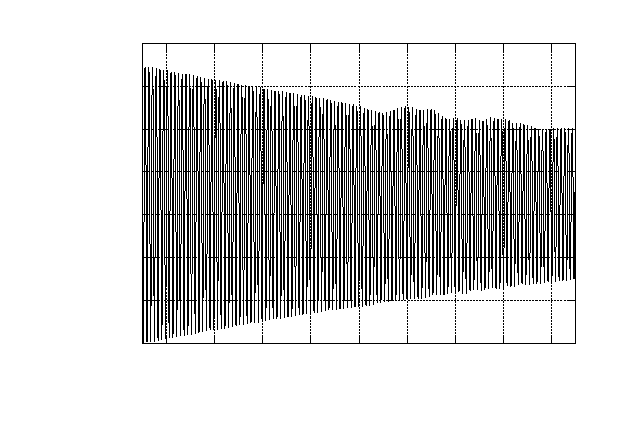
\includegraphics{./CrazyEnergy}}%
    \gplfronttext
  \end{picture}%
\endgroup

\end{figure}
}

\frame{
\begin{figure}
% GNUPLOT: LaTeX picture with Postscript
\begingroup
  \makeatletter
  \providecommand\color[2][]{%
    \GenericError{(gnuplot) \space\space\space\@spaces}{%
      Package color not loaded in conjunction with
      terminal option `colourtext'%
    }{See the gnuplot documentation for explanation.%
    }{Either use 'blacktext' in gnuplot or load the package
      color.sty in LaTeX.}%
    \renewcommand\color[2][]{}%
  }%
  \providecommand\includegraphics[2][]{%
    \GenericError{(gnuplot) \space\space\space\@spaces}{%
      Package graphicx or graphics not loaded%
    }{See the gnuplot documentation for explanation.%
    }{The gnuplot epslatex terminal needs graphicx.sty or graphics.sty.}%
    \renewcommand\includegraphics[2][]{}%
  }%
  \providecommand\rotatebox[2]{#2}%
  \@ifundefined{ifGPcolor}{%
    \newif\ifGPcolor
    \GPcolortrue
  }{}%
  \@ifundefined{ifGPblacktext}{%
    \newif\ifGPblacktext
    \GPblacktexttrue
  }{}%
  % define a \g@addto@macro without @ in the name:
  \let\gplgaddtomacro\g@addto@macro
  % define empty templates for all commands taking text:
  \gdef\gplbacktext{}%
  \gdef\gplfronttext{}%
  \makeatother
  \ifGPblacktext
    % no textcolor at all
    \def\colorrgb#1{}%
    \def\colorgray#1{}%
  \else
    % gray or color?
    \ifGPcolor
      \def\colorrgb#1{\color[rgb]{#1}}%
      \def\colorgray#1{\color[gray]{#1}}%
      \expandafter\def\csname LTw\endcsname{\color{white}}%
      \expandafter\def\csname LTb\endcsname{\color{black}}%
      \expandafter\def\csname LTa\endcsname{\color{black}}%
      \expandafter\def\csname LT0\endcsname{\color[rgb]{1,0,0}}%
      \expandafter\def\csname LT1\endcsname{\color[rgb]{0,1,0}}%
      \expandafter\def\csname LT2\endcsname{\color[rgb]{0,0,1}}%
      \expandafter\def\csname LT3\endcsname{\color[rgb]{1,0,1}}%
      \expandafter\def\csname LT4\endcsname{\color[rgb]{0,1,1}}%
      \expandafter\def\csname LT5\endcsname{\color[rgb]{1,1,0}}%
      \expandafter\def\csname LT6\endcsname{\color[rgb]{0,0,0}}%
      \expandafter\def\csname LT7\endcsname{\color[rgb]{1,0.3,0}}%
      \expandafter\def\csname LT8\endcsname{\color[rgb]{0.5,0.5,0.5}}%
    \else
      % gray
      \def\colorrgb#1{\color{black}}%
      \def\colorgray#1{\color[gray]{#1}}%
      \expandafter\def\csname LTw\endcsname{\color{white}}%
      \expandafter\def\csname LTb\endcsname{\color{black}}%
      \expandafter\def\csname LTa\endcsname{\color{black}}%
      \expandafter\def\csname LT0\endcsname{\color{black}}%
      \expandafter\def\csname LT1\endcsname{\color{black}}%
      \expandafter\def\csname LT2\endcsname{\color{black}}%
      \expandafter\def\csname LT3\endcsname{\color{black}}%
      \expandafter\def\csname LT4\endcsname{\color{black}}%
      \expandafter\def\csname LT5\endcsname{\color{black}}%
      \expandafter\def\csname LT6\endcsname{\color{black}}%
      \expandafter\def\csname LT7\endcsname{\color{black}}%
      \expandafter\def\csname LT8\endcsname{\color{black}}%
    \fi
  \fi
    \setlength{\unitlength}{0.0500bp}%
    \ifx\gptboxheight\undefined%
      \newlength{\gptboxheight}%
      \newlength{\gptboxwidth}%
      \newsavebox{\gptboxtext}%
    \fi%
    \setlength{\fboxrule}{0.5pt}%
    \setlength{\fboxsep}{1pt}%
\begin{picture}(5760.00,3844.00)%
    \gplgaddtomacro\gplbacktext{%
      \csname LTb\endcsname%
      \put(946,704){\makebox(0,0)[r]{\strut{}$-200$}}%
      \csname LTb\endcsname%
      \put(946,1023){\makebox(0,0)[r]{\strut{}$0$}}%
      \csname LTb\endcsname%
      \put(946,1343){\makebox(0,0)[r]{\strut{}$200$}}%
      \csname LTb\endcsname%
      \put(946,1662){\makebox(0,0)[r]{\strut{}$400$}}%
      \csname LTb\endcsname%
      \put(946,1982){\makebox(0,0)[r]{\strut{}$600$}}%
      \csname LTb\endcsname%
      \put(946,2301){\makebox(0,0)[r]{\strut{}$800$}}%
      \csname LTb\endcsname%
      \put(946,2621){\makebox(0,0)[r]{\strut{}$1000$}}%
      \csname LTb\endcsname%
      \put(946,2940){\makebox(0,0)[r]{\strut{}$1200$}}%
      \csname LTb\endcsname%
      \put(946,3260){\makebox(0,0)[r]{\strut{}$1400$}}%
      \csname LTb\endcsname%
      \put(946,3579){\makebox(0,0)[r]{\strut{}$1600$}}%
      \csname LTb\endcsname%
      \put(1316,484){\makebox(0,0){\strut{}$-80$}}%
      \csname LTb\endcsname%
      \put(1792,484){\makebox(0,0){\strut{}$-60$}}%
      \csname LTb\endcsname%
      \put(2268,484){\makebox(0,0){\strut{}$-40$}}%
      \csname LTb\endcsname%
      \put(2744,484){\makebox(0,0){\strut{}$-20$}}%
      \csname LTb\endcsname%
      \put(3221,484){\makebox(0,0){\strut{}$0$}}%
      \csname LTb\endcsname%
      \put(3697,484){\makebox(0,0){\strut{}$20$}}%
      \csname LTb\endcsname%
      \put(4173,484){\makebox(0,0){\strut{}$40$}}%
      \csname LTb\endcsname%
      \put(4649,484){\makebox(0,0){\strut{}$60$}}%
      \csname LTb\endcsname%
      \put(5125,484){\makebox(0,0){\strut{}$80$}}%
    }%
    \gplgaddtomacro\gplfronttext{%
      \csname LTb\endcsname%
      \put(176,2141){\rotatebox{-270}{\makebox(0,0){\strut{}$E$}}}%
      \put(3220,154){\makebox(0,0){\strut{}$\tau$}}%
    }%
    \gplbacktext
    \put(0,0){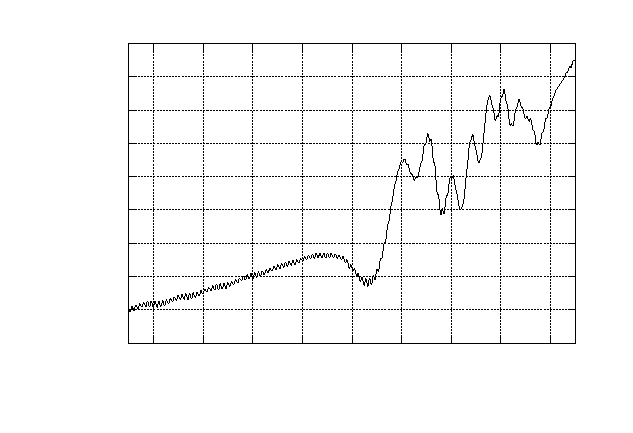
\includegraphics{./GoodEnergy}}%
    \gplfronttext
  \end{picture}%
\endgroup

\end{figure}
}


\end{document}